\section{Clasificación de Eventos Físicos: \\ Eventos Task y Eventos Happening}
\label{sec:clasificacion_eventos_fisicos} 

El monitor de RdP es el único responsable del bloqueo o habilitación de un hilo
que ejecuta una acción emisora de eventos físicos de salida. El hilo realiza el
disparo de petición de ejecución al inicio de la ejecución del programa, sin
tener en cuenta el estado actual de la red (ver
sección~\ref{sec:sincronizacion_peticion_ejecucion}). En consecuencia, el hilo
queda bloqueado en el monitor hasta que el mismo decide desbloquearlo,
dependiendo del estado de la red y la política de prioridades (ver
Figura~\ref{fig:actividades_evento_task}).

\begin{figure}[H]
	\centering
	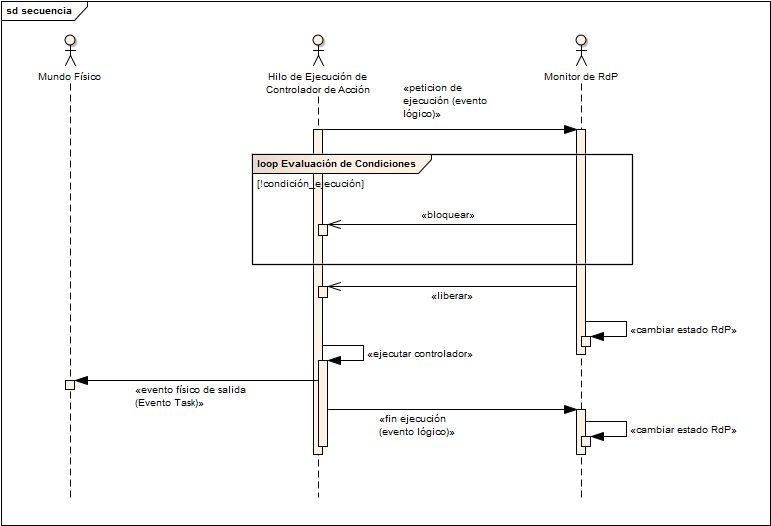
\includegraphics[width=0.9\textwidth]{secuencia_evento_task}
	\caption{Diagrama de Secuencia de la Ejecución de una Acción que Emite un
	Evento Físico de Salida}
	\label{fig:actividades_evento_task}
\end{figure}

En la Figura~\ref{fig:actividades_evento_happening} se observa que
la ejecución de una acción encargada de recibir un evento físico de entrada
depende, en primera instancia de la ocurrencia de dicho evento. Luego, también
es sincronizada con la RdP mediante el uso del monitor. De este modo, las
acciones que reciben eventos físicos de entrada presentan una restricción extra
respecto a aquellas que emiten eventos físicos de salida.



\begin{figure}[H]
	\centering
	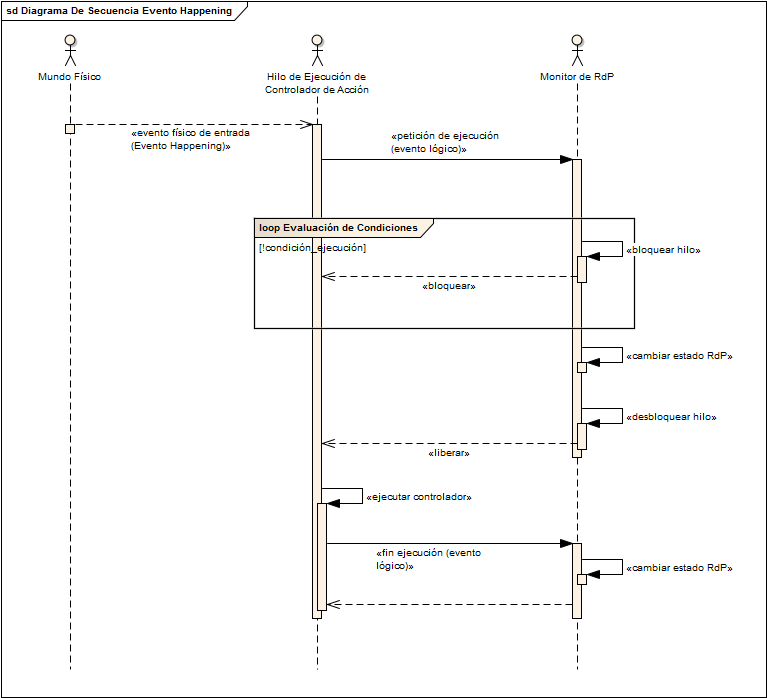
\includegraphics[width=0.9\textwidth]{secuencia_evento_happening}
	\caption{Diagrama de Secuencia de la Ejecución de una Acción que Recibe un
	Evento Físico de Entrada}
	\label{fig:actividades_evento_happening}
\end{figure}

Desde este punto de vista, se decidió dar una clasificación más significativa a
los eventos físicos. Esta clasificación estará presente a lo largo de todo
el desarrollo del framework.
\begin{itemize}
  \item Eventos Task (Tarea): Eventos físicos de salida. Son
  desencadenados y sincronizados exclusivamente por eventos lógicos que dependen
  de condiciones ya presentes en el monitor de Redes de Petri al momento de su
  emisión. Si bien el monitor no produce directamente eventos físicos, puede
  advertirse que un evento task tiene una relación directa con determinados
  eventos lógicos. Dichos eventos lógicos se encuentran definidos en un tópico
  (evento de acción).
  \item Eventos Happening (Suceso): Eventos físicos de entrada. Son
  desencadenados por el mundo externo de manera totalmente asincrónica respecto
  al sistema. La ejecución de las acciones que reciben y manejan estos eventos
  es sincronizada por el monitor de redes de petri. De esta forma, el monitor
  conserva su responsabilidad frente al manejo del asincronismo del sistema.
  Los eventos lógicos requeridos para la sincronización se encuentran definidos
  en un tópico (evento de acción).
\end{itemize}

\section{Controladores de Acciones: \\ Task Controllers y Happening Controllers}
\label{sec:controladores_de_acciones}

Las acciones que debe realizar el sistema, junto con las interfaces necesarias
para la comunicación de los eventos físicos correspondientes, se encuentran
embebidos dentro de controladores de acción. En la
Figura~\ref{fig:arquitectura_petri-manejador-acciones-mundo} se muestran dichos
controladores.\\

A partir de la clasificación de eventos físicos propuesta en la
sección~\ref{sec:clasificacion_eventos_fisicos}, surge la necesidad de
clasificar los controladores de acción respecto a su condición de receptores de
Eventos Happening, o de emisores de Eventos Task. En consecuencia, emerge un
nuevo requerimiento del framework, relacionado con el requerimiento número 2
definido en la sección~\ref{sec:definicion_reqs}:
\begin{itemize}
    \item El framework debe ofrecer interfaces para especificar si un
    controlador de acción responde a un evento físico de entrada o a un
    evento físico de salida.
\end{itemize}
En respuesta a este requerimiento se definen los controladores de tipo
Happening Controller y Task Controller.

\subsection{Ejecución de un Task Controller}
\label{sec:ejecucion_task_controller}
De acuerdo al diseño del framework, el comportamiento dinámico de los eventos
Task es dirigido únicamente por la evolución de los estados de la RdP. Esto se
debe a las siguientes condiciones:
\begin{itemize}
    \item En la sección~\ref{sec:resumen_sincronizacion} se explicita que el
    modo de sincronización adoptado es el de petición de ejecución al monitor. De
    esta forma se admiten disparos asíncronos a transiciones realizados desde
    diferentes hilos de ejecución, delegando en el monitor la responsabilidad de
    bloquear los hilos que no cumplen con las condiciones necesarias para la ejecución.

    \item En la sección~\ref{sec:clasificacion_eventos_fisicos} se determina la
    existencia de una relación directa entre un Evento Task y un conjunto de
    eventos lógicos.

    \item Un Evento Task es desencadenado por condiciones que estan presentes en el
    monitor al momento de la emisión de este evento
\end{itemize}

Del analisis anterior emerge un nuevo requerimiento, relacionado
con el requerimiento 2 de la sección~\ref{sec:definicion_reqs}:
\begin{itemize}
    \item El framework debe ser responsable de crear y controlar la
    ejecución de los hilos de ejecución para controladores de acción que
    generan eventos físicos de salida.
\end{itemize}

 Como corolario, se determina que la ejecución de un Task Controller debe
 encapsularse en un hilo al momento de inicialización del programa. El hilo se
 encarga de:
\begin{enumerate}
  \item Realizar las peticiones de los permisos de sincronización al
  monitor de forma directa, sin tener en cuenta el estado de la red.
  \item  Ejecutar el código correspondiente al Task Controller, una vez que el
  monitor otorga el permiso.
  \item  Realizar el aviso de finalización de ejecución al monitor de Petri.
  \item Repetir los pasos de ejecución de forma infinita, delegando en el
  monitor el control de la ejecución.
\end{enumerate}

La responsabilidad de la creación de los hilos para ejecutar los Task
Controllers pertenece al framework. En consecuencia, la ejecución de las
acciones encapsuladas en un Task Controller es transparente al usuario
desarrollador.

\begin{figure}[H]
	\centering
	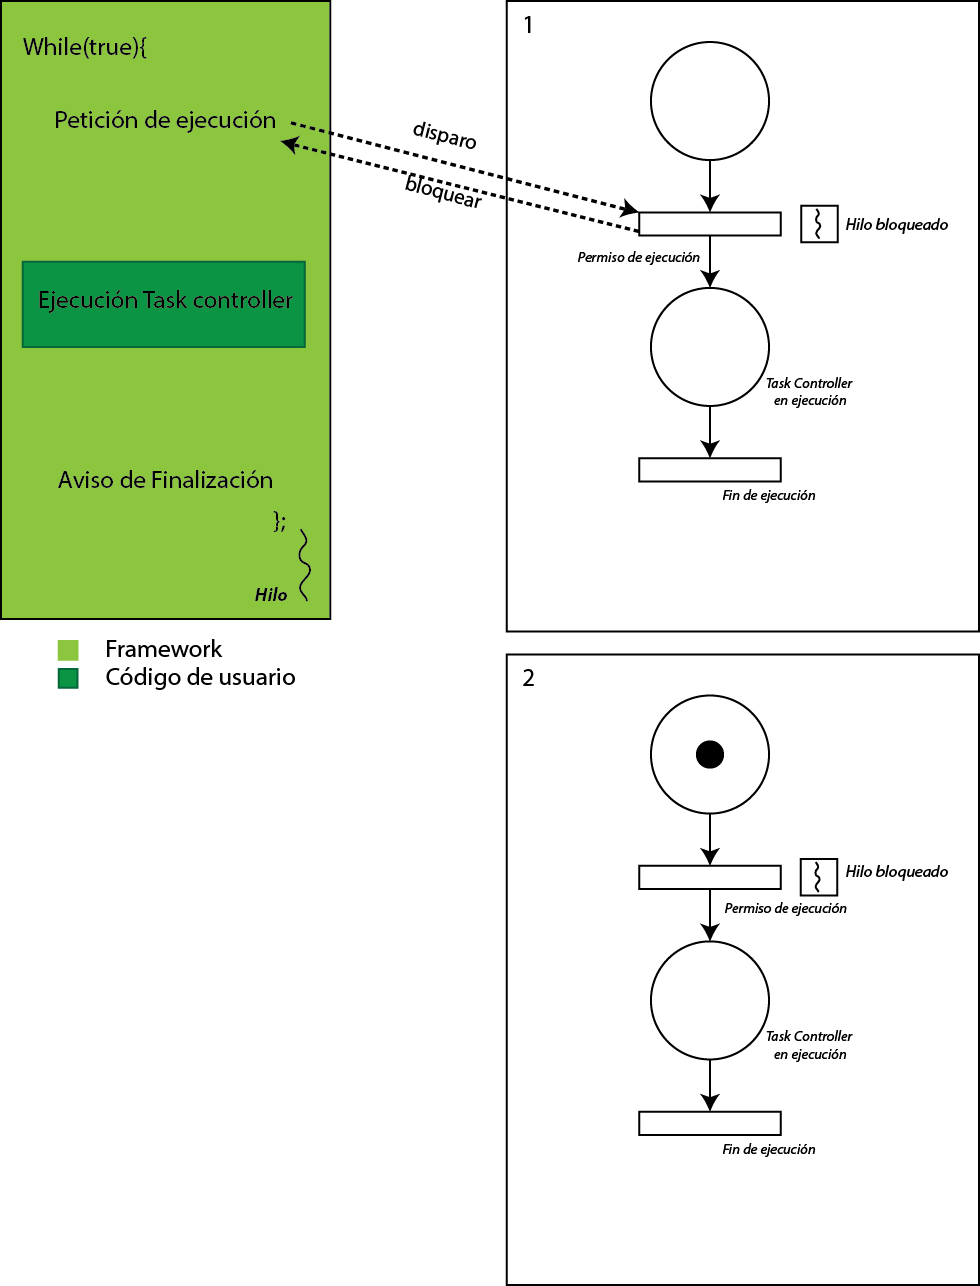
\includegraphics[width=0.9\textwidth]{ejecucion_task_controller_pt1}
\end{figure}
\begin{figure}[H]
	\centering
	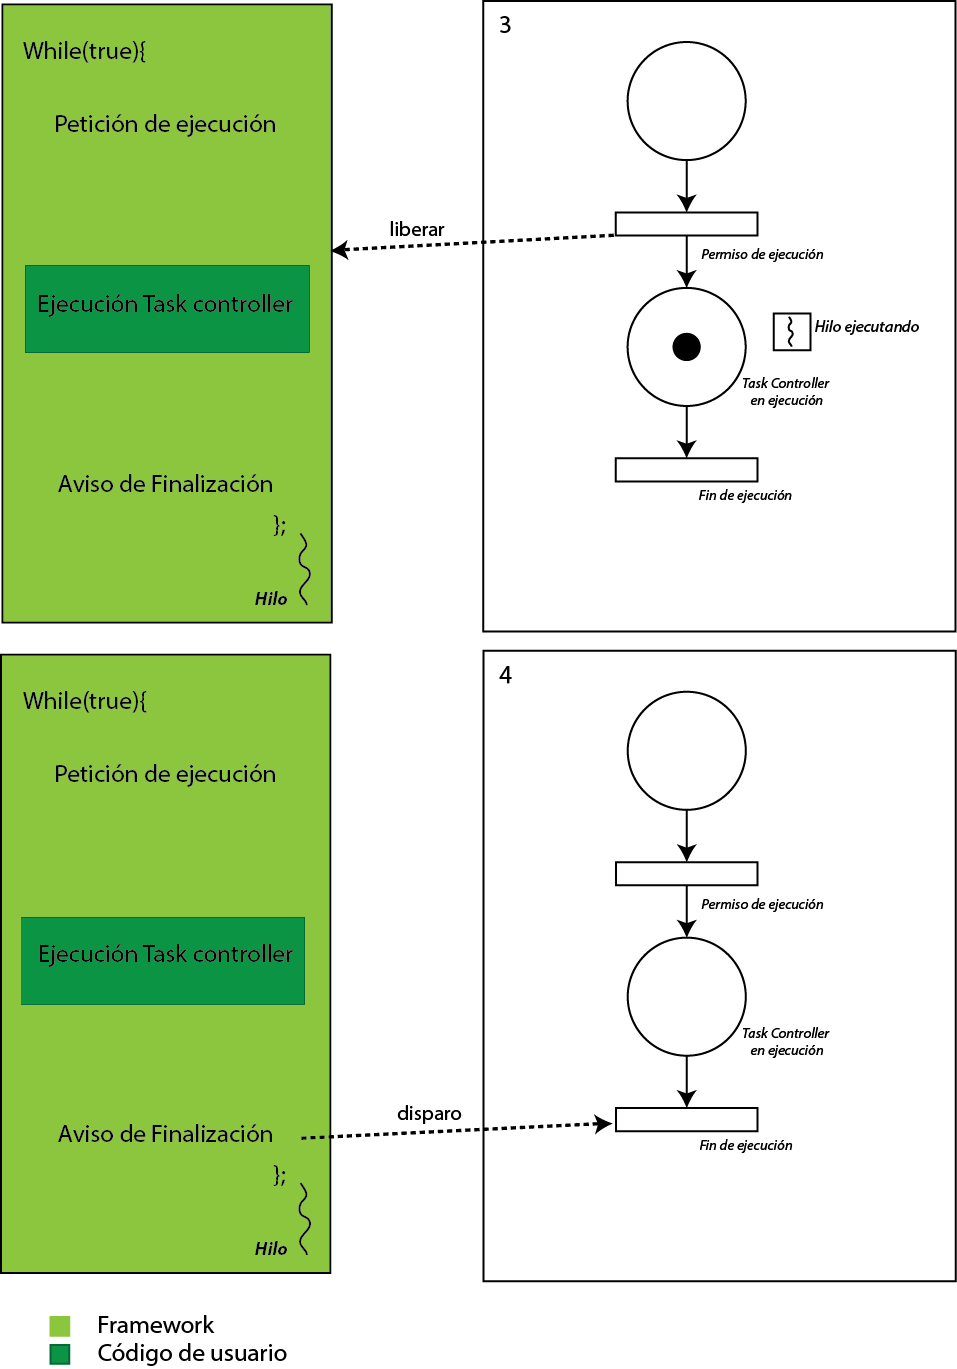
\includegraphics[width=0.9\textwidth]{ejecucion_task_controller_pt2}
	\caption{Pasos de la Ejecución de un Task Controller}
	\label{fig:ejecucion_task_controller}
\end{figure}

\newpage

\subsection{Ejecución de un Happening Controller}
\label{sec:ejecucion_happening_controller}
Un Evento Happening se desencadena en el mundo externo y de forma asíncrona al
sistema (ver sección~\ref{sec:clasificacion_eventos_fisicos}). 
En consecuencia, el código de usuario es responsable de realizar la llamada a
ejecución de un Happening Controller, encargado de manejar dicho evento.

En principio, realizar una llamada desde el código de usuario podría generar un
grave problema en cuanto a las responsabilidades de sincronización. Las
acciones del Happening Controller quedarían fuera del mecanismo de
sincronización del monitor de Petri, atentando contra el objetivo de delegar
el asincronismo del sistema en la RdP. \\

Del análisis anterior emerge un nuevo requerimiento, relacionado con el
requerimiento 2 de la sección~\ref{sec:definicion_reqs}:
    \begin{itemize}
        \item El framework debe ser responsable de controlar la ejecución de los
        hilos creados por el usuario, correspondientes a controladores de acción
        que manejan eventos físicos de entrada.
    \end{itemize}

Este requerimiento se cumple mediante la utilización de herramientas de la
programacón orientada a aspectos (ver sección~\ref{sec:aop}). Se optó por
encapsular las instrucciones de sincronización necesarias dentro de advices.
Dichos advices son aplicados en joinpoints, definidos por los puntos de
ejecución del programa donde existen llamadas a ejecución o retornos de
rutinas de tipo Happening Controller.

\begin{framed}
\textbf{Nota:}
	Un controlador de acción que reacciona ante
	eventos Happening (Happening Controller) debe ser ejecutado dentro del
	contexto de un Listener u Observer del evento deseado.
	Para maximizar las libertades de elección del desarrollador en la recepción de
	eventos externos, la responsabilidad de crear estos Listeners se delega en el
	usuario.
\end{framed}


El flujo de ejecución de un Happening Controller es el siguiente:
\begin{enumerate}
  \item Cuando el código de usuario hace un llamado a la ejecución del Happening
  Controller, la aplicación alcanza un joinpoint.
  \item En el momento en que se alcanza el joinpoint se aplica un advice que
  realiza los pedidos de permiso de sincronización al monitor. Dicho advice es
  aplicado automáticamente en tiempo de compilación, por lo tanto el usuario no
  tiene la responsabilidad de realizar la sincronización manualmente. De esta
  manera se logra conservar la inversión de control.
  \item Una vez que el monitor libera el hilo, indicando que la ejecución es
  posible, se procede a ejecutar el código del controller.
  \item Al finalizar la ejecución del Happening Controller, se alcanza un nuevo
  joinpoint.
  \item En el momento en que se alcanza el joinpoint descripto en el punto
  anterior se aplica un advice que realiza el aviso de finalización de
  ejecución al monitor. Este advice se aplica de manera análoga a la descripta
  en el punto 2.
\end{enumerate}

\begin{framed}
\textbf{Nota:} Los advices descriptos en esta sección son ejecutados por el
mismo hilo que ejecuta el código del Happening Controller. Dado que la llamada
al código del Happening Controller es responsabilidad del usuario, es él quien
debe generar el hilo encargado de ejecutar el código. Se recomienda no utilizar
el hilo principal del programa para ejecutar Happening Controllers ya que puede
ocasionar el bloqueo del sistema.
\end{framed}

En conclusión, la sincronización de la ejecución de los Happening Controllers
sigue siendo una responsabilidad del monitor y es realizada de forma
transparente al usuario. Es posible realizar La llamada a un HappeningController
en cualquier punto del código de la aplicación, de esta forma el usuario
tiene libertad para realizar el manejo de eventos físicos de entrada. Se destaca
que aunque el usuario tiene la libertad de llamar al código del Happening
Controller en cualquier momento, el monitor es responsable de determinar si
la ejecución del controlador comenzará al momento de la llamada a ejecución, o
si bloqueará el hilo por no cumplirse las condiciones de ejecución del controlador.

\begin{figure}[H]
	\centering
	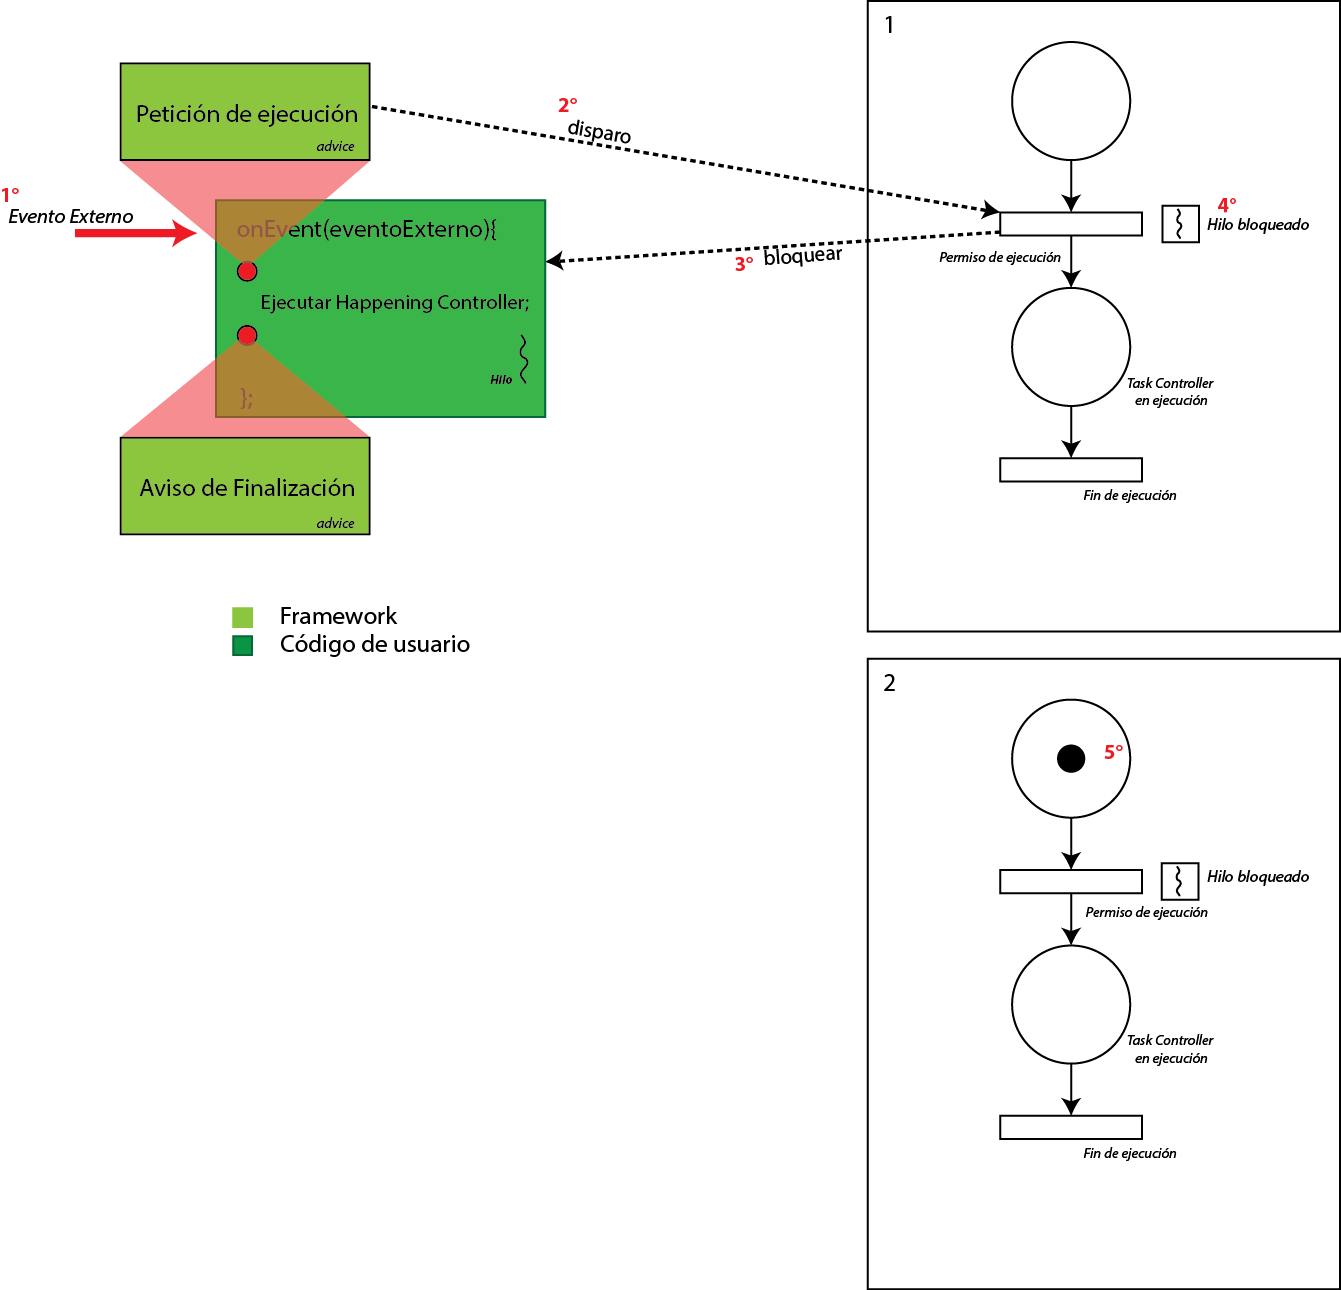
\includegraphics[width=0.9\textwidth]{ejecucion_happening_controller_pt1}
\end{figure}
\begin{figure}[H]
	\centering
	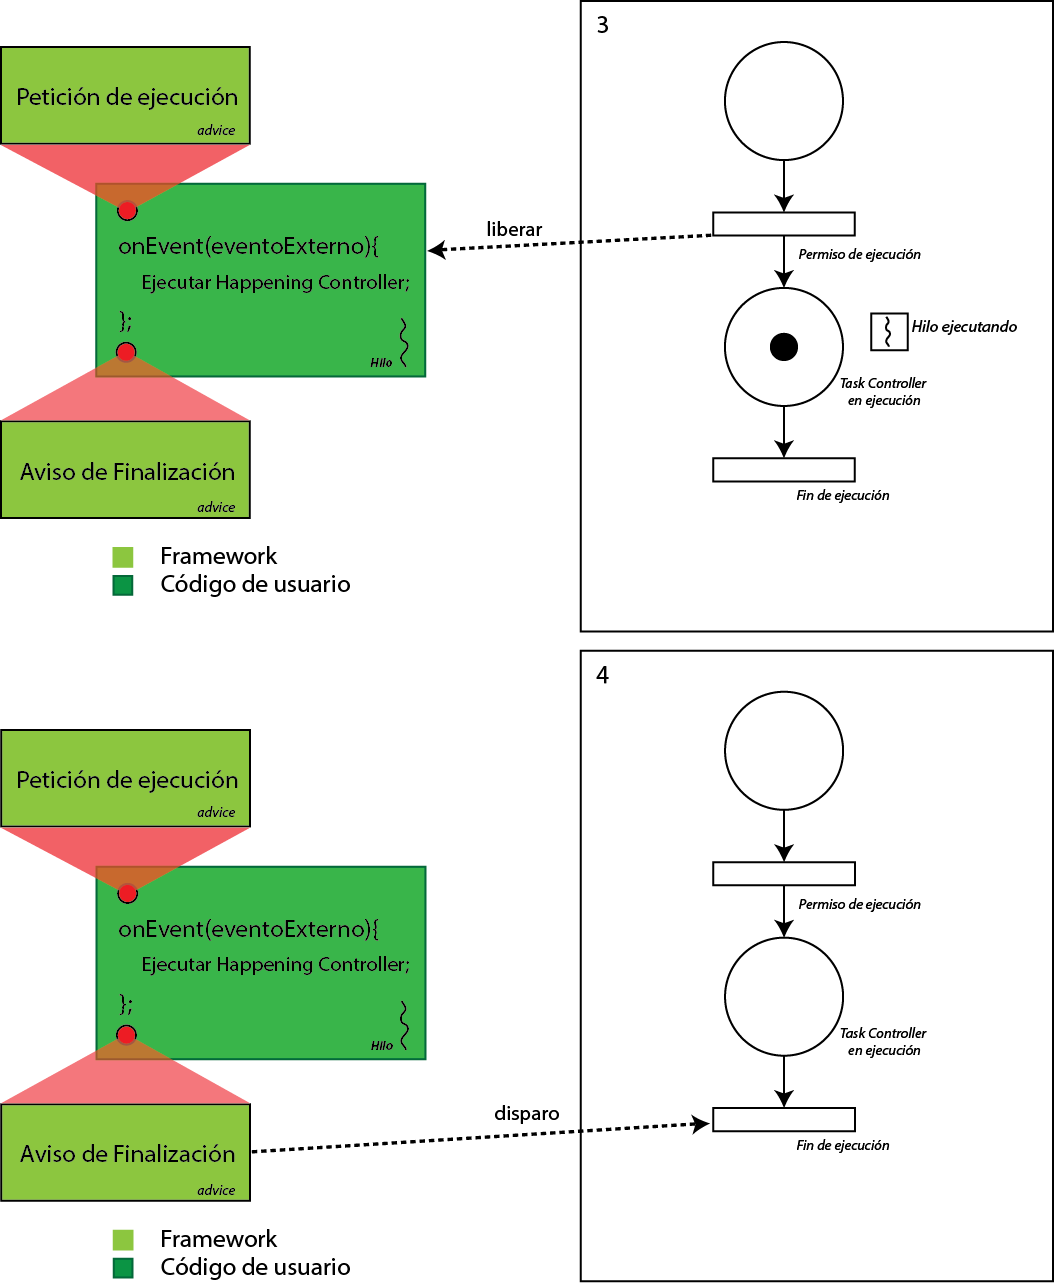
\includegraphics[width=0.75\textwidth]{ejecucion_happening_controller_pt2}
	\caption{Pasos de la Ejecución de un Happening Controller}
	\label{fig:ejecucion_happening_controller}
\end{figure}

\section{ComplexSequentialTaskController}
\label{sec:complex_sequential_task_controller}
En esta sección se presenta una optimización de la ejecución de Task Controllers
(ver sección~\ref{sec:ejecucion_task_controller}) para sistemas de caracter
secuencial, como el que se estudia en la
sección~\ref{sec:sincronizacion_cinta_transportadora}.
Debido a que no existe un paralelismo aprovechable en una secuencia de
tareas dependientes resulta innecesario utilizar un hilo
por cada Task Controller correspondiente a cada tarea secuencial.

En respuesta a este problema, se determinó que los Task Controllers de acciones
correspondientes a un proceso secuencial deben ser ejecutados por un mismo hilo.
Esta agrupación de controladores se denomina Complex Sequential Task
Controller.
\\
La utilización de Complex Sequential Task Controllers reduce la
cantidad de hilos necesarios para ejecutar un sistema con tareas secuenciales.
Para lograrlo, se incorpora una etapa de petición de permisos y una etapa de
ejecución de controlador por cada Task Controller que forma parte del
ComplexSequentialTaskController. Cada una de estas etapas debe seguir el orden
preestablecido por la secuencia de acciones que conforman el proceso secuencial.
Dicho orden se establece en el tópico, al definir el evento de acción para la
sincronización de la tarea compleja.

Una ventaja de agrupar tareas secuenciales en un mismo hilo es que permite
eliminar la plaza-transición incorporada por el Modo de Sincronización de
petición de de ejecución (ver sección~\ref{sec:sincronizacion_peticion_ejecucion_transicion_plaza}).

\begin{figure}[H]
	\centering
	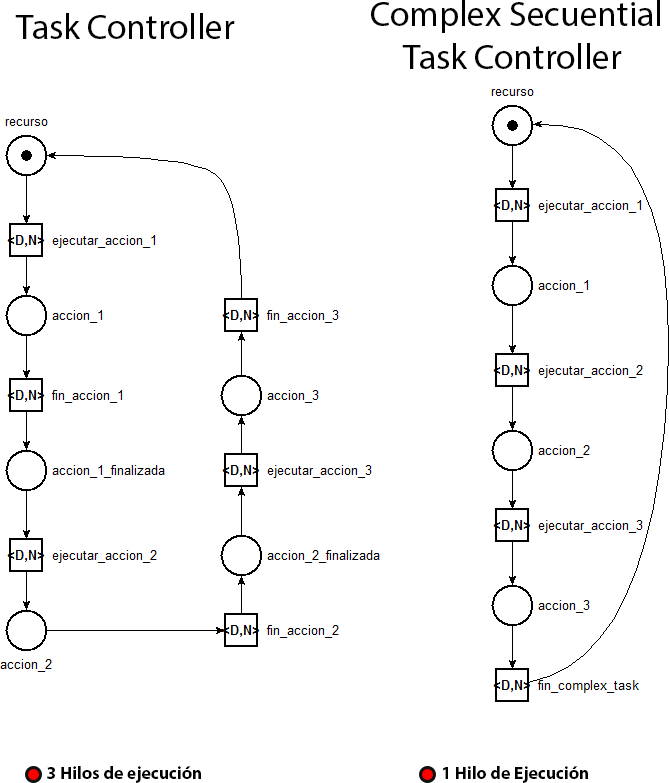
\includegraphics[width=0.8\textwidth]{simple_vs_complex_task_petri_net}
	\caption{Comparación del modelo en RdP de un sistema con tres
	acciones secuenciales para Task Controllers simples y para Complex Sequential
	Task Controller.}
	\label{fig:simple_task_vs_complex_task_petri_net}
\end{figure}

\begin{figure}[H]
	\centering
	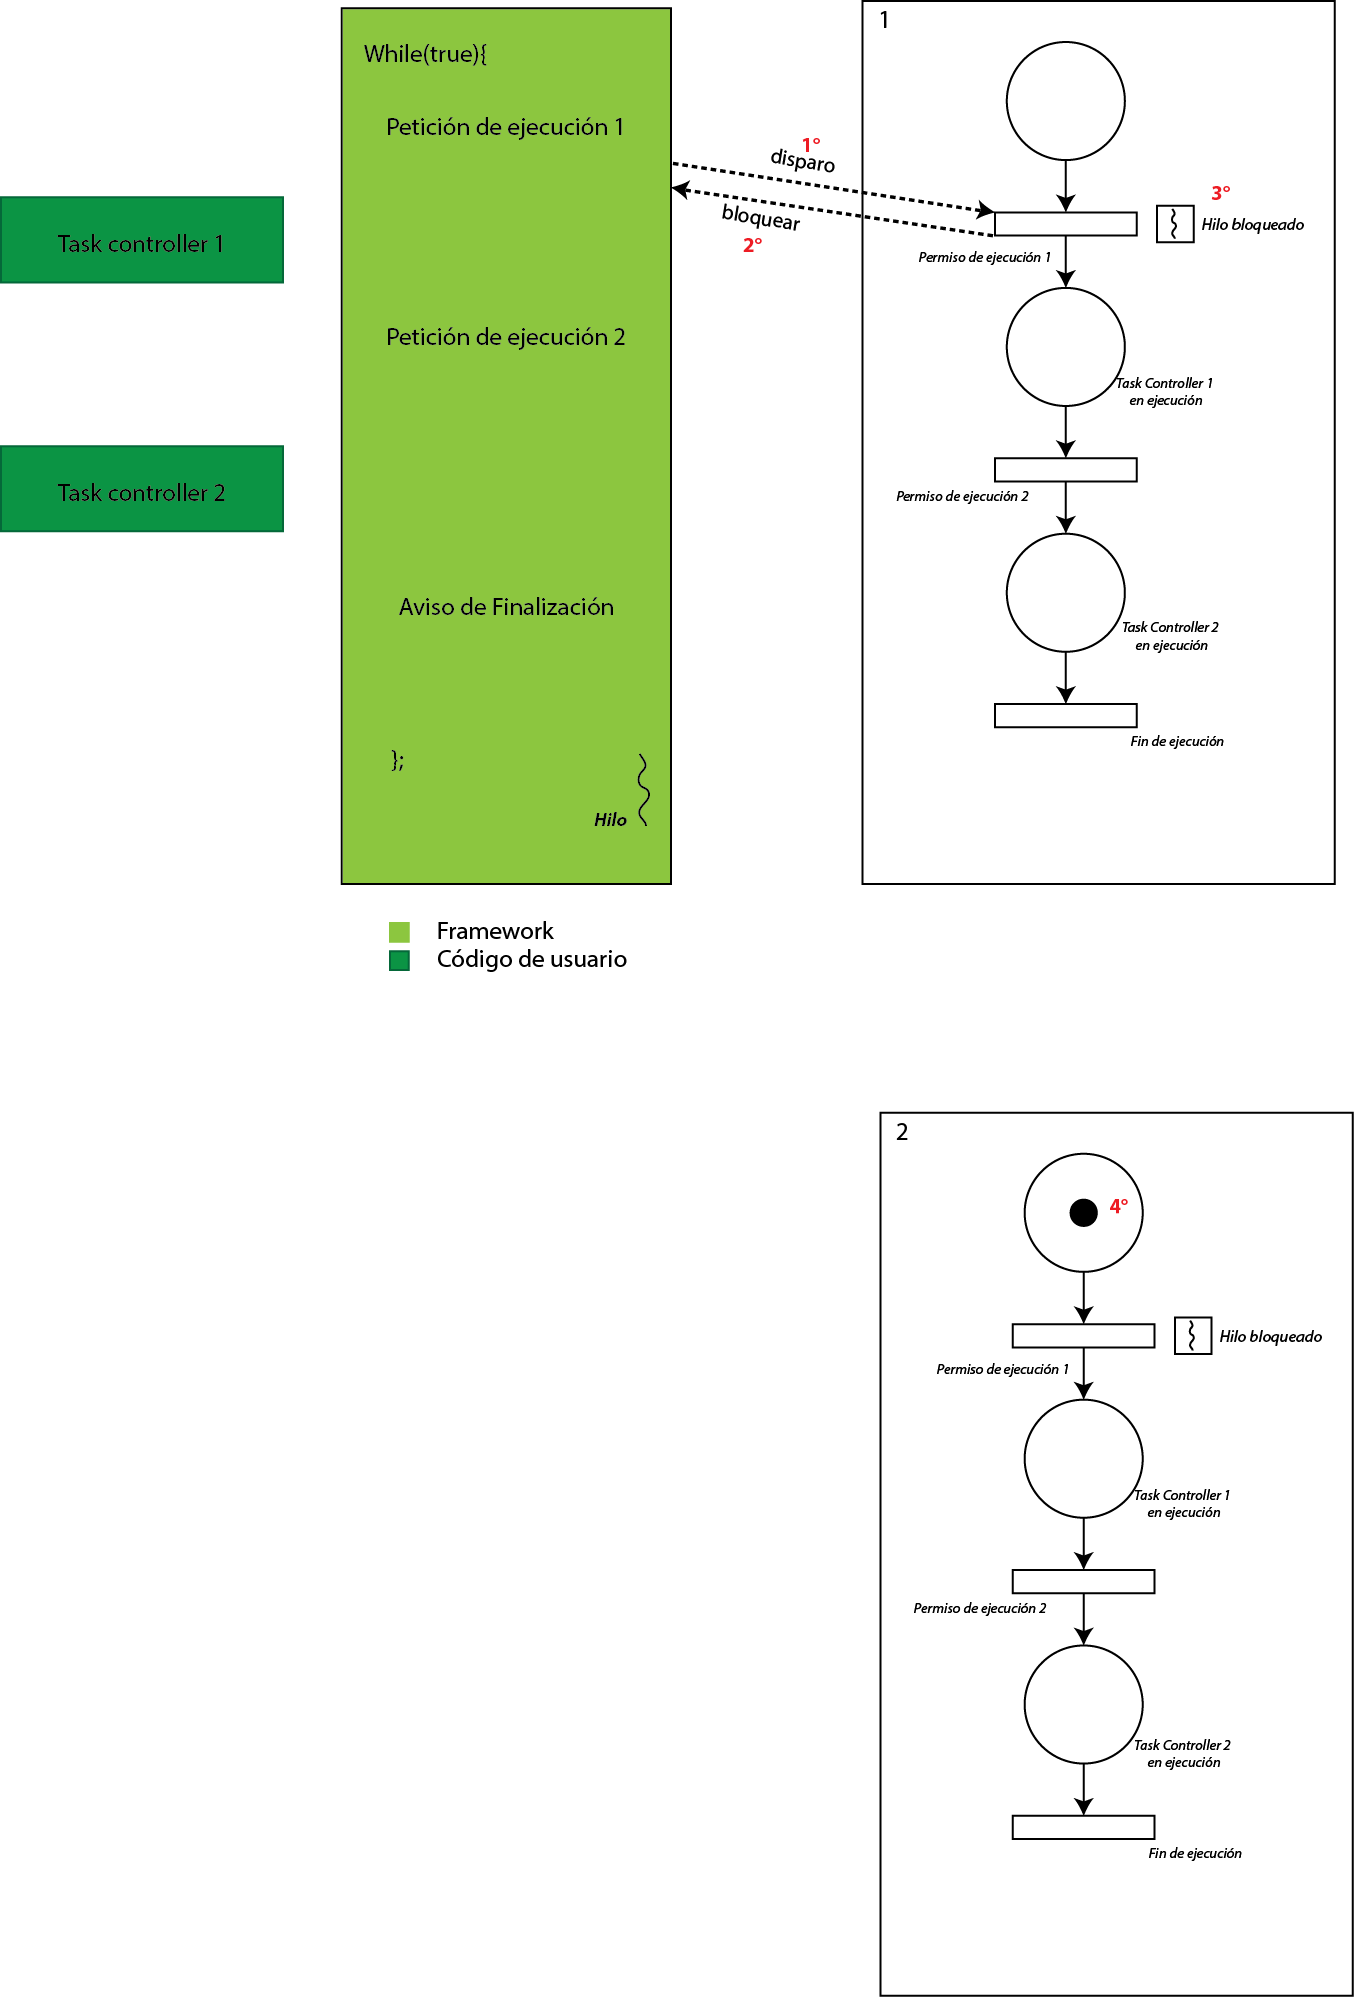
\includegraphics[width=0.9\textwidth]{ejecucion_complextask_controller_pt1}
\end{figure}

\begin{figure}[H]
	\centering
	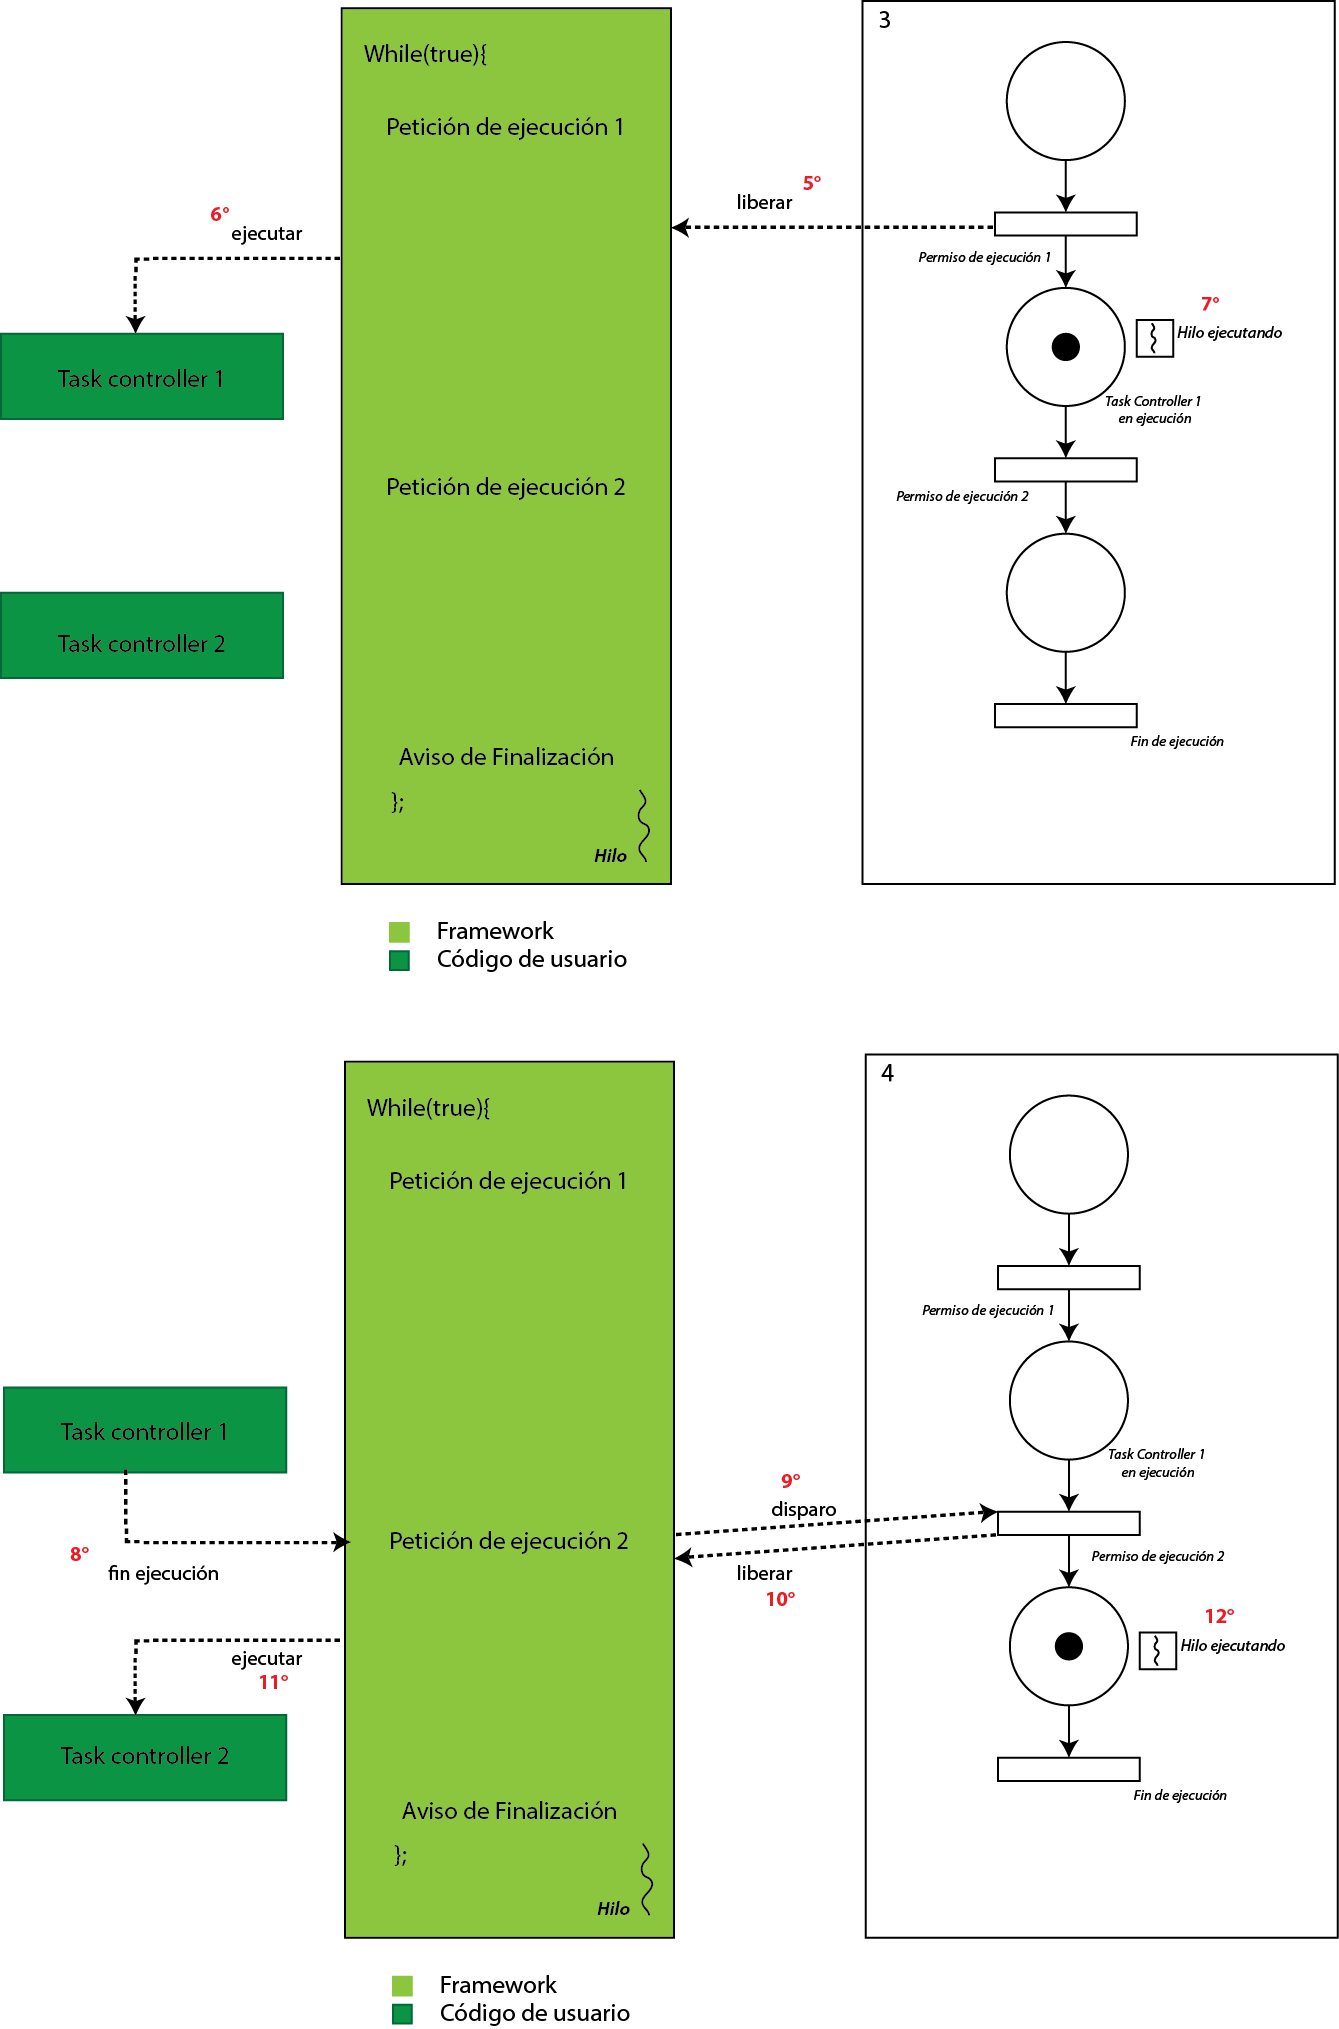
\includegraphics[width=0.9\textwidth]{ejecucion_complextask_controller_pt2}
\end{figure}

\begin{figure}[H]
	\centering
	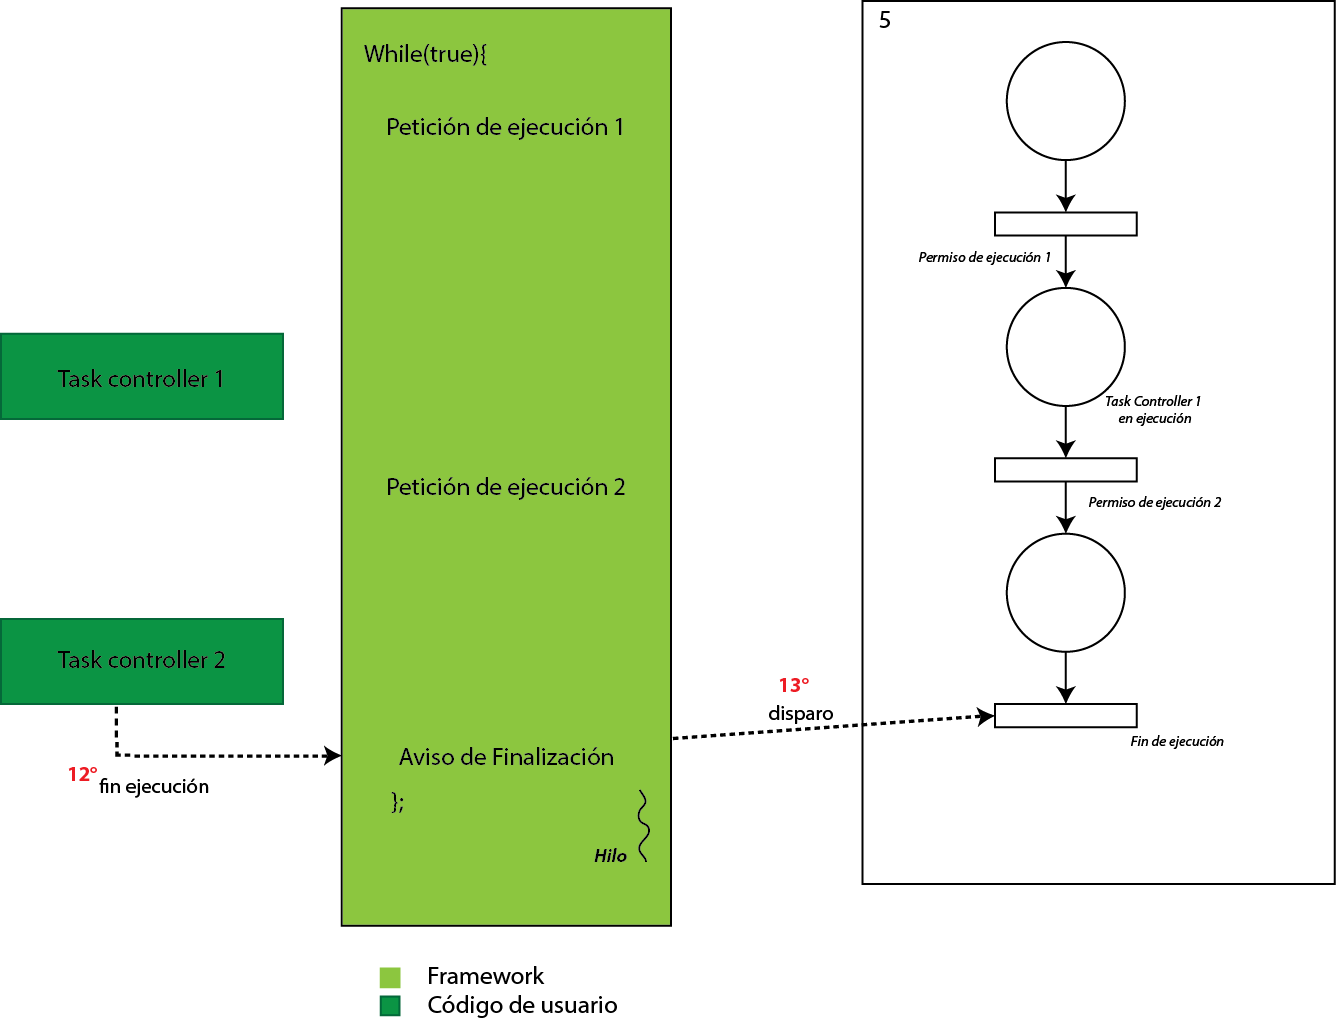
\includegraphics[width=0.9\textwidth]{ejecucion_complextask_controller_pt3}
	\caption{Pasos de la Ejecución de un Complex Sequential Task Controller con
	Dos Acciones Task}
	\label{fig:ejecucion_complextask_controller}
\end{figure}